\documentclass{beamer}
%\usepackage{lstlisting}
\title{Image Steganography with FPGA}
\author{Aithu Snehith, Nakka Chakradhar}
\date{}
\begin{document}

\begin{frame}
\titlepage
\end{frame}

%\begin{frame}
%	\tableofcontents
%\end{frame}


\section{Introduction to FPGA}
\frame{
\frametitle{Introduction to FPGA}
A field-programmable gate array (FPGA) is an integrated circuit designed to be configured by a customer or a designer after manufacturing – hence the term "field-programmable". The FPGA configuration is generally specified using a hardware description language (HDL)
\newline
Generally there are licensed tool-chains to program and work with FPGAs. Here we are exploring icoprog - an opensource FPGA bitstream convertor for FPGAs.
}

\section{Introduction}
\frame{
\frametitle{Introduction to Steganography}
Steganography is the practice of concealing a file(any information) within another file.

}
\section{Project Scope}
\frame{
\frametitle{Project Scope}

This project is useful for hiding information  in any file.
The scope of the project is implementing steganography on FPGAs for hiding information which includes any type of files like image files, audio files, video, apk etc., in any other file.
\vspace{5mm} \newline
For this project we're hiding a message string in an image file.
}

\section{Methodology}
\frame{
\frametitle{Methodology - LSB insertion}

The LSB is the lowest significant bit in the byte value of the character.
\vspace{5mm} \newline
The LSB based image steganography hides the secret(byte) in the least significant bits of pixel values of the cover image.
\begin{figure}[t!]
    \centering
    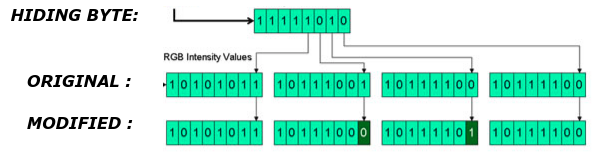
\includegraphics[width=0.6\textwidth]{lsb.png}
    \caption{Overview of LSB Insertion}
\end{figure}
}

\section{Rundown on Algorithm}
\frame{
\frametitle{Rundown on Algorithm}
Here is a quick rundown on the algorithm we're implementing here
\begin{figure}[t!]
    \centering
    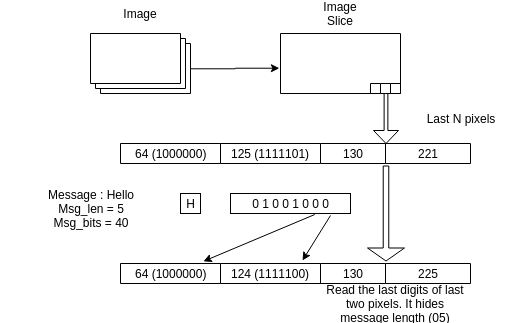
\includegraphics[width=0.8\textwidth]{alru.png}
    \caption{Overview of LSB Insertion}
\end{figure}
}

\section{Hardware Connections}
\frame{
\frametitle{Hardware Connections}
A quick look on the connections we're making between Raspi, FTDI and IcoBoard
\begin{figure}[t!]
    \centering
    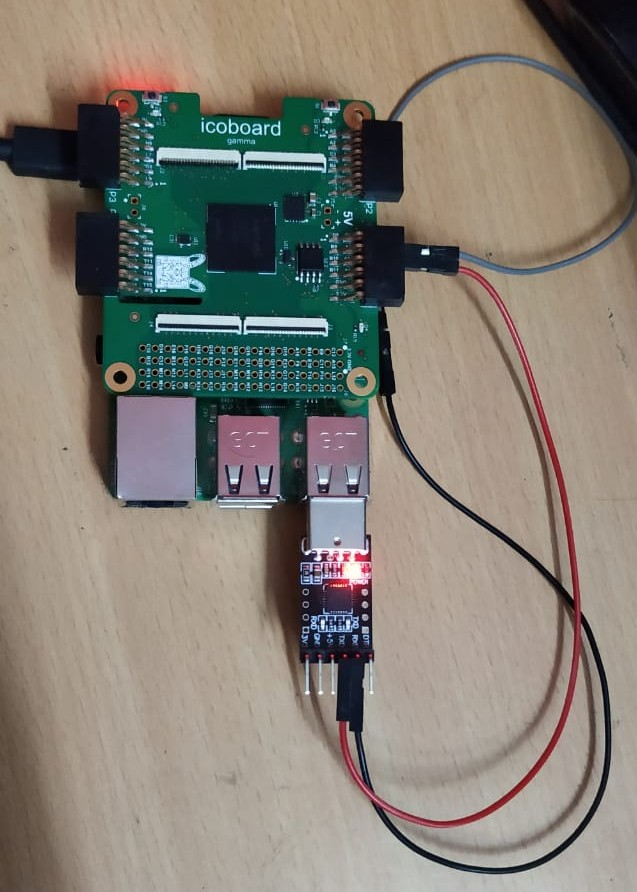
\includegraphics[width=0.5\textwidth, angle=90]{or.jpeg}
    \caption{Overview of LSB Insertion}
\end{figure}
}


\section{Installation of open-source tools}
\frame{
\frametitle{Installation of open-source tools}
We would require 4 tools primarily to work with FPGAs
\begin{itemize}
    \item Icestorm
    \item Arachne-PNR
    \item Yosys
    \item Icoprog
\end{itemize}

These are all available for Linus systems. We'd be primarily dealing with Ubuntu based systems
}

\section{Installation of Dependencies}
\frame{
\frametitle{Installation of Dependencies}
For the above 4 tools to work, first we need to install the following dependencies
\begin{itemize}
    \item sudo apt install build-essential clang bison flex 
    \item sudo apt install libreadline-dev gawk tcl-dev libffi-dev 
    \item sudo apt install git mercurial graphviz xdot pkg-config 
    \item sudo apt install python python3 libftdi-dev qt5-default 
    \item sudo apt install python3-dev libboost-all-dev cmake
\end{itemize}
run the command as it is on a terminal session
}


\section{Icestorm installation}
\frame{
\frametitle{Icestorm}
\begin{itemize}
\item git clone https://github.com/cliffordwolf/icestorm.git icestorm
\item cd icestorm
\item make -j\$(nproc)
\item sudo make install
\end{itemize}
}

\section{Arachne installation}
\frame{
\frametitle{Arachne-PNR}
\begin{itemize}
\item git clone https://github.com/cseed/arachne-pnr.git arachne-pnr
\item cd arachne-pnr
\item make -j\$(nproc)
\item sudo make install
\end{itemize}
}

\section{Yosys Installation}
\frame{
\frametitle{Yosys}
\begin{itemize}
\item git clone https://github.com/cliffordwolf/yosys.git yosys
\item cd yosys
\item make -j\$(nproc)
\item sudo make install
\end{itemize}
}

\section{Icoprog Installation}
\frame{
\frametitle{Icoprog Installation}
These steps must be done on Raspi as these are to burn the .bin to IcoBoard

\begin{itemize}
\item cd \$HOME
\item git clone git://git.drogon.net/wiringPi
\item cd wiringPi \&\& ./build
\vspace{0.5cm}
\item cd \$HOME
\item sudo apt-get install subversion
\item svn co http://svn.clifford.at/handicraft/2015/icoprog
\item cd icoprog \&\& make install
\end{itemize}
}

\section{Implementation}
\frame{
\frametitle{UART in Verilog}
We are deploying two verilog modules for this purpose
\begin{itemize}
\item UART protocol to send out the encoded image
\item Module to hide any given text in the pixel matrix of the image
\end{itemize} 
}

\section{Implementation details}
\frame{
\frametitle{Contents of each file}
Lets dive into the code for better understanding
\begin{itemize}
\item v\_gen.py - generates the required .v file by accepting image and message string as inputs
\item steg.pcf - a pin configuration file. We can change what pins act Rx and Tx for the UART
\item regen\_img.py - receives input from IcoBoard and spits out image mod.png with string hidden inside
\item decrypt.py - decrypts and reconstruct the hidden message from the image mod.png
\end{itemize} 
}

\section{Execution}
\frame{
\frametitle{How to execute - Laptop}
Here are the steps for execution
\begin{itemize}
\item run the command python v\_gen.py. The command asks you to enter message and image name. Enter accordingly
\item run $make$ in terminal to generate verilog file. It is suggested to do it on a laptop or system as the compilation takes a lot of time on Raspberry pi.
\item If run on a laptop, copy the files onto Raspberry Pi by some sorts.
\item If Raspi is on a local network, copy the files from laptop with the following command - $scp$ $steg.bin$ pi@ip\_addr:$path$
\item run $icoprog -p < steg.bin$ on Raspi to flash the bin file
\item Run regen\_img.py on Raspi to receive and save the encrypted image
\item Run decrypt.py to decrypt and display the message
\end{itemize} 
}

\section{Execution}
\frame{
\frametitle{How to execute - Raspberry}
Here are the steps for execution
\begin{itemize}
\item run the command python v\_gen.py. The command asks you to enter message and image name. Enter accordingly
\item run $make$ in terminal to generate verilog file
\item run $icoprog -p < steg.bin$ on Raspi to flash the bin file
\item Run regen\_img.py on Raspi to receive and save the encrypted image
\item Run decrypt.py to decrypt and display the message
\end{itemize} 
}

\section{Execution}
\frame{
\frametitle{TL:DR ? Shorter way of execution}
Here are the steps for execution
\begin{itemize}
\item Run sh build.sh on Laptop to build the bin file and push it to raspberry pi on the local network
\item Run execute\_nd\_decrypt.sh to decrypt and display the message
\end{itemize} 
}

\section{Changes after LSB Insertion}
\frame{
\frametitle{Changes After LSB Insertion}
Comparing two images before and after hiding text shows that there is no significant visual changes in the image
\begin{figure}[t!]
    \centering
    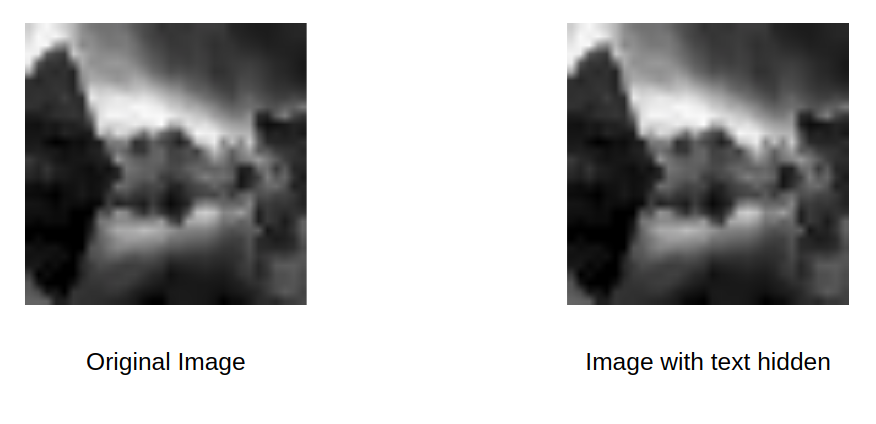
\includegraphics[width=0.5\textwidth]{change.png}
    \caption{Comaprision after LSB Insertion}
\end{figure}
}


\section{Alternative Methods}
\frame{
\frametitle{Alternative Method}
Although this is not a viable approach, another alternative way to solve this problem is to deploy a PicoRV32 as an SoC onto IcoBoard and do the computations.
\vspace*{1cm}
Once PicoRV32 is implimented, we can run RISC-V GCC compatible C codes. So instead of generating Verilog files with image matrices, we generate C codes and compile and flash onto icoboard. The compilation takes time so it's adviced to run it on a Laptop
}

\section{Alternative Methods}
\frame{
\frametitle{Alternative Method}
Another advantage to this method is once the processing is done, PicoRV32 has comm modules pre-defined which we can use by configuring PMOD pins. One notable example is UART.
\vspace*{1cm}
Not just that but once PicoRV32 is implemented, Raspi assumes access to one of the registers on the IcoBoard which enables console output. So we can use printf statements in the above mentioned C code for debugging or Raw communication purposes.
}

\section{References}
\frame{
\frametitle{References}
\begin{itemize}
\item ZipCPUs implementation of UART - https://github.com/ZipCPU/icozip/tree/master/rtl
\item CliffordWolf Icotools - https://github.com/cliffordwolf/icotools
\item Pramode's Blog posts on working with IcoBoards and UART - http://pramode.in/2016/10/05/fpga-programming-with-foss-tools/
\item Google search for FTDI functionality
\end{itemize}
}


\end{document}
